\begin{enumerate}[label=\thesection.\arabic*.,ref=\thesection.\theenumi]
\numberwithin{equation}{enumi}

\item Using Nyquist criterion, find out the range of K for which the closed loop system will be stable.\newline
\begin{align}
\label{eq:es17btech11015_system}
    \nonumber G(s)=\frac{K}{(s+1)(s+3)}
    \\
    H(s)=\frac{1}{(s+5)(s+7)}
\end{align}

\item The system flow can be described by Fig. \ref{fig:es17btech11015_fig1}
\begin{figure}[!ht]
    \begin{center}
        \resizebox{\columnwidth}{!}{%\begin{figure}
\tikzstyle{block} = [draw, fill=blue!20, rectangle, 
        minimum height=1cm, minimum width=1cm]
\tikzstyle{sum} = [draw, fill=blue!20, circle, node distance=1cm]
\tikzstyle{input} = [coordinate]
\tikzstyle{output} = [coordinate]
\tikzstyle{pinstyle} = [pin edge={to-,thin,black}]
    
    % The block diagram code is probably more verbose than necessary
\begin{tikzpicture}[auto, node distance=2cm,>=latex']
    % We start by placing the blocks
    \node [input, name=input] {X(s)};
    \node [sum, right of=input] (sum) {};
    \node [block, right of=sum] (system) {$\frac{K}{(s+1)(s+3)}$};
    %\node [block, right of=controller] (system) {$K$};
        % We draw an edge between the controller and system block to 
        % calculate the coordinate u. We need it to place the measurement block. 
%    \draw [->] (system) -- node[name=u] {} (system);
    \node [output, right of=system] (output) {};
    \node [block, below of=system] (measurements) {$\frac{1}{(s+5)(s+7)}$};
    
    % Once the nodes are placed, connecting them is easy. 
    \draw [draw,->] (input) -- node {$X(s)$} (sum);
    \draw [->] (sum) -- node {} (system);
    \draw [draw,->] (system) -- node [name=y] {$Y(s)$}(output);
    \draw [->] (y) |- (measurements);
    \draw [->] (measurements) -| node[pos=0.99] {$-$} 
        node [near end] {} (sum);
\end{tikzpicture}
%\end{figure}}
    \end{center}
    \caption{}  
    \label{fig:es17btech11015_fig1}
\end{figure}
\item Find the open loop transfer function G(s)H(s)
\\
\solution From \eqref{eq:es17btech11015_system},
%
 \begin{align}
 \label{eq:es17btech11015_openloop}
L(s)=G(s)H(s)&=\frac{K}{(s+1)(s+3)(s+5)(s+7)}
 \end{align}
 \begin{align}
L(j\omega)=G(\j \omega)H(\j \omega)=\frac{K}{(j\omega+1)(j\omega+3)(j\omega+5)(j\omega+7)}
\end{align}

\item Sketch the Nyquist plot.
\\
\solution The Nyquist plot is a graph of $\text{Re} \cbrak{L(jw)}$  vs $\text{Im} \cbrak{L(j\omega)}$.
Let's take K=1 and draw the nyquist plot.
\\

The following python code generates the Nyquist plot.
\begin{lstlisting}
    /codes/es17btech11015.py
\end{lstlisting}
%
The  Fig.  \ref{fig:es17btech11015} shows the Nyquist plot for K = 1 
\begin{figure}[!h]
  \centering
  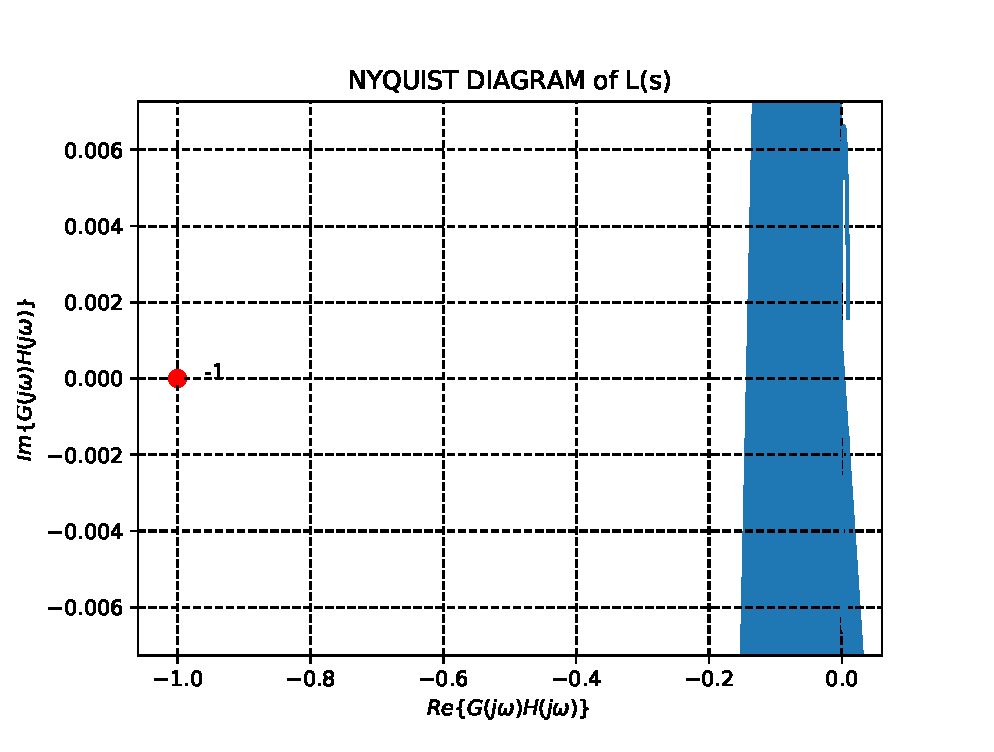
\includegraphics[width=\columnwidth]{./figs/es17btech11015.eps}
  \caption{}
  \label{fig:es17btech11015}
\end{figure}

\item  Using the Nyquist Stability criterion, determine the value of K for which the system in \eqref{eq:es17btech11015_system} is stable.
\\
\solution  \\\textbf{Nyquist criterion}-For the stable system :
\begin{align}
\label{eq:es17btech11015_nyquist}
Z = P+N = 0,    
\end{align}
where, 
\\
Z = Poles of $\frac{G(s)}{1+G(s)H(s)} $  in right half of s plane
\\

P = Poles of $G(s)H(s) $ in right half of s plane
\\

N = No. of encirclements of $G(s)H(s)$ about -1 in the Nyquist plot
\\

Since from the equation \eqref{eq:es17btech11015_openloop}, P = 0 
\\

So, for Z to be equal to 0 ,we have to choose the range of K such that N is equal to 0.
\\
\item Find the range of K from Nyquist criterion.
\solution From the figure \ref{fig:es17btech11015}, we can observe that the plot is not cutting the x-axis. If we consider the Nyquist plot with K term even then the plot won't cut the x-axis. 
\\
So, N = 0 irrespective of K. 
\\
Therefore, the system is stable for 
\begin{align}
    -\infty < K < \infty
\end{align}

\end{enumerate}
